\chapter{Vektorbündel}
\section{Tangentialbündel}
Wir wollen nun alle Tangentialräume einer Mannigfaltigkeit $\mfk$ gemeinsam betrachten.
\begin{align}
T\mfk = \bigcup_{p\in \mfk} T_{p}\mfk = \{ (p, V) \vert p \in \mfk, v \in T_{p}\mfk \} 
\end{align}
Wir wollen nun die Struktur einer differenzierbaren Mannigfaltigkeit. 
Das heißt wir müssen eine Topologie und eine $\cinf$-Struktur auf $T\mfk$ definieren.
\begin{align}
\pi: T\mfk &\to \mfk \\
(p,V) &\mapsto p
\end{align}
Sei $(x, U)$ eine Karte von $\mfk^m$. 
Dann definieren wir eine Karte $(\overline{x}, \overline{U})$ von $T\mfk$ wie folgt:
\begin{align}
&\overline{U} = \pi^{-1}(U) = \bigcup_{p\in\mfk} T_{p}\mfk \\
&\overline{x}: \overline{U} \to x(U) \times \R^m \subset \R^{2m} \\
&(p, V) \mapsto (x(p), \xi)
\end{align}

\begin{figure}[h]
\centering
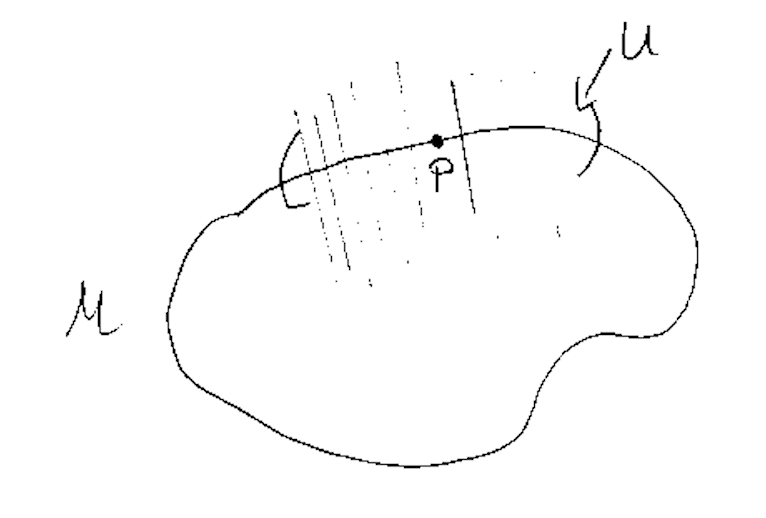
\includegraphics[width=0.4\linewidth]{figures/scan/tangentialbuendel.png}
\caption{Veranschaulichung eines Tangentialbündels}
\label{img:tangentialbuendel}
\end{figure} 

Wobei $\xi = (\xi^1, \dots, \xi^m) \in \R^m$ gegeben ist durch:
\begin{align}
v = \sum_{i=1}^{m} \xi_i \pdv{x_i} \big\vert_p, \quad \forall p \in U.
\end{align}
Wir haben noch keine Topologie auf $T\mfk$ definiert, das heißt $\overline{x}$ ist nur eine bijektive Abbildung zwischen Mengen.
Wir können allerdings nicht sagen ob es ein Homöomorphismus oder Diffeomorphismus ist.
Allerdings können wir Kartenwechsel betrachten.\\
Seien $(\overline{x}, \overline{U})$ und $(\overline{y}, \overline{U}')$ zwei Karten. 
Betrachte die Abbildungen:
\begin{align}
\overline{y} \circ \overline{x}^{-1} \circ \underbrace{x (\overline{U} \cap \overline{U}')}_{x(U \cap U') \times \R^m} \to \underbrace{\overline{y}(\overline{U} \cap \overline{U}')}_{y(U \cap U') \times \R^m}
\end{align}
\begin{align}
(x,\xi) \mapsto (y\circ x^{-1}(U), \eta) 
\end{align}
Wobei $\eta = \dd (y \circ x^{-1})\big\vert_U \xi$.\\
Da $y\circ x^{-1}$ Diffeomorphismus ist, ist $\overline{y} \circ \overline{x}^{-1}$ ein Isomorphimus.
Nun können wir die Topologie auf $T\mfk$ definieren.
$O \subset T\mfk$ offen, falls $\overline{x}(O\cap \overline{U})$ offen in $V \times \R^m$ ist für alle Karten $(x, U) \in \atlas_\mfk$ (bzw $(\overline{x}, \overline{U}) \in \atlas_{T\mfk}$)
\begin{satz}
$T\mfk$ mit dieser Topologie ist eine topologische Mannigfaltigkeit und $\atlas_{T\mfk}$ eine differenzierbare Struktur.
\end{satz}
\section{Vektorbündel}
$T\mfk$ hat die Struktur einer glatten Mannigfaltigkeit.
Allerdings hat es noch mehr, nämchlich die eines Vektorbündels, was wir nun definieren.
\begin{defs}[Vektorbündel]
Sei $\mfk$ eine differenzierbare Mannigfaltigkeit.
Ein $\R$-Vektorbündel vom $\rang$ $k$ über $\mfk$ ist eine differenzierbare Mannigfaltigkeit mit einer glatten surjektiven Abbildung:
\begin{align}
\pi: E \to \mfk,
\end{align}
so dass:
\begin{enumerate}
\item $\forall p \in \mfk$ hat $E_p:= \pi^{-1}( \{ p \})$ die Struktur eines $\R$-Vektorraums der Dimension $k$.
$E_p$ heißt Faser von $E$ über $p$.
\item Für alle $p$ in $\mfk$ existiert eine Umgebung $U$ von $p$ in $\mfk$ und ein Diffeomorphismus.
\begin{align}
\begin{xy}
\xymatrix@=0.2\linewidth{
      \phi: U \times \R^k \ar[rr] \ar[rd]_{pr_1}  &     &  \pi^{-1}(U) \ar[dl]^{\pi}  \\
                             &  U  &}
\end{xy}
\end{align}
%\begin{figure}[h]
%\centering
%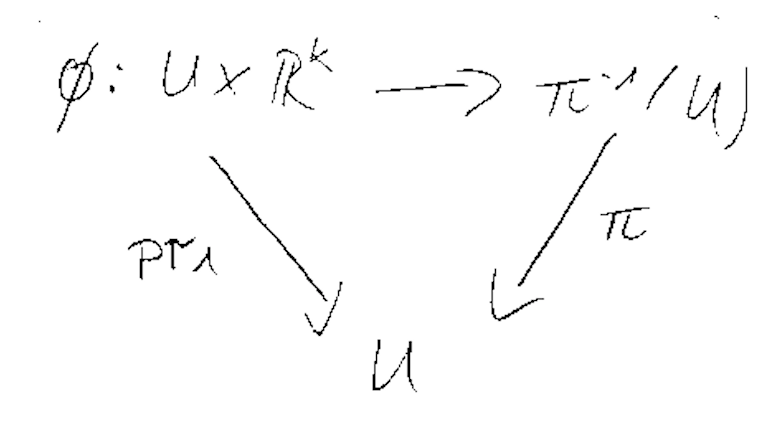
\includegraphics[width=0.4\linewidth]{figures/scan/lokaletrivialisierung.png}
%\caption{Lokale Trivialisierung}
%\label{img:lokaletrivialisierung}
%\end{figure} 
Für diesen gilt:
\begin{itemize}
\item $\pi \circ \phi = p r_1$
\item Für alle $q \in U$ ist die Abbildung
\begin{align}
\phi\big\vert_q : \{ q \} \times \R^k &\to E_q\\
\{ q, \xi \} &\mapsto \phi_q (\xi) := \phi(q, \xi)
\end{align}
$\phi$ heißt lokale Trivialisierung von $E$.
\end{itemize}
\end{enumerate}
\end{defs}
\begin{bem}
Ein Vektorbündel ist ein Tripel $(\pi, E, \mfk)$ aber wir schreiben oft nur $E$. Hierbei wird $E$ Totalraum und $\mfk$ Basis genannt.
\end{bem}
\begin{bsp} \leavevmode
\begin{enumerate}
\item Triviale Bündel:
\begin{align}
&E = \mfka \times \R^k \to \mfk\\
&(p, \xi) \mapsto p
\end{align}
\item Tangentialbündel 
\begin{align}
&\pi: T\mfk \to \mfk\\
&(p, V) \to V
\end{align}
\item Tautologisches Bündel
\begin{align}
&\mfk = \R \mathbb{P}^n\\
&E = \{ (l, x) \vert l \in \R \mathbb{P}^n, x\in l \subset \R^{n+1} \}\\
&\pi: E \to \mfk = \R \mathbb{P}^n\\
&(l, x) \mapsto l
\end{align}
Behauptung: Dies ist ein Vektorbündel vom $\rang$ $1$.
Vektorraumstruktur auf $E_l$:
\begin{align}
(l, x) + (l, y) &:= (l, x + y)\\
k (l, x) &:= (l, k x)
\end{align}
\end{enumerate}
\end{bsp}
Nun wollen wir uns damit beschäftigen wie wir Vektorbündel konstruieren können.
Angenommen uns wäre das folgende gegeben:
\begin{enumerate}
\item $E_p, p\in \mfk$ eine Familie von Vektorräumen der Dimension $k$
\item $(U_\alpha)_{\alpha \in \atlas}$ eine offene Überdeckung von $\mfk$
\item $\forall \alpha \in \atlas$, $p\in U_\alpha$ gibt es den folgenden Isomorphismus:
\begin{align}
\phi_{\alpha, p}: \R^\alpha \to E_p
\end{align}
\end{enumerate}
Setze 
\begin{align}
&E = \cup_{p \in \mfk} E_p\\
&\pi : E \to \mfk\\
&(p, V) \mapsto p\\
&\phi_\alpha: U_\alpha \times \R^k \to E \big\vert_{U_\alpha}\\
&(p, \xi) \mapsto (p, \phi_{\alpha, p}(\xi)).
\end{align}
Nun stellt sich die Frage unter welchen Vorraussetzungen $(\pi, E, \mfk)$ ein Vektorbündel ist.
\begin{lem}
\label{lem:vorraussetzungenvektorbündel}
Sei $\mfk$ eine glatte Mannigfaltigkeit, $E$ eine Menge und die Abbildung $\pi: E\to\mfk$ surjektiv.
Sei $\{ U_\alpha \}$ eine offene Überdeckung von $\mfk$ zusammen mit bijektiven Abbildungen
\begin{align}
\phi^{-1}_{\alpha} = \varphi: \pi^{-1}(U_\alpha) \to U_\alpha \times \R^\alpha,
\end{align}
die $pr_1 \circ \varphi_\alpha = \pi$ erfüllen, so dass wann immer $U_\alpha \cap U_\beta \neq \emptyset$, dann ist 
\begin{align}
\varphi_\alpha \circ \varphi_{\beta}^{-1} \to (U_\alpha \cap U_\beta) \times \R^k,
\end{align}
von der Form:
\begin{align}
\label{eq:konstruktionvektorbündel}
(\varphi_\alpha \circ \varphi_{\beta}^{-1})(p, v) = (p, \tau(p) v)
\end{align}
mit einer glatten Abbildung $\tau: U_\alpha \cap U_\beta \to \mathrm{GL}(k, \R)$.
Dann existiert eine eindeutige Struktur als glattes $k$-dim Vektorbündel über $\mfk$ für die $\varphi^{-1}_{\alpha}$ lokale Trivialisierungen sind.
\end{lem}
\begin{bew}[Beweis Lemma \ref{lem:vorraussetzungenvektorbündel}]
Sei  $p\in\mfk$. 
Setze $E_p := \pi^{-1}(\{ p \})$. 
Falls $p\in U_\alpha$, dann ist 
\begin{align}
\varphi_\alpha \big\vert_p : E_p \to \{ p \} \times \R^k.
\end{align}
Definiere eine Vektorraumstruktur auf $E_p$ durch die Forderung, dass die Abbildung $\varphi_\alpha \big\vert_p$ ein Isomorphismus ist.
Durch verkleinern von $U_\alpha$ und hinzunahme von weiteren offenen Mengen kann man annehmen, dass jedes $U_\alpha$ diffeomorph zu $\overline{U}_\alpha \subseteq \R^m$ ist.
Verknüpfung von $\varphi_\alpha$ mit einem solchen Diffeomorphismus liefert eine Bijektion:
\begin{align}
\pi^{-1} (U_\alpha) \to \overline{U}_\alpha \times \R^k .
\end{align}
Diese nutzen wir als Karte für $E$.
Wegen Gleichung \ref{eq:konstruktionvektorbündel} bekommen wir eine glatte Struktur auf $E$.
\end{bew}
Sei $(x, U)$ Karte von $\mfk$, $p\in U$, $v\in T_p \mfk$.
\begin{align}
v = \sum_{i=1}^{m} \xi_i \pdv{x_i}\big\vert_p
\end{align}
Definiere:
\begin{align}
\varphi: \pi^{-1} (U) &\to U \times \R^m\\
v &\mapsto (p, V)
\end{align}
Dort wo $(x)$ und $(\overline{x})$ überlappen.
\begin{align}
\pdv{x_i} \big\vert_p &= (\pdv{\overline{x}_j}{x_i})\pdv{\overline{x}_j} \big\vert\\
v &= \sum_{j=1}^{m} \xi_j \pdv{\overline{x}_j}  \big\vert_p = \sum_{ji1}^{m} \xi_i \pdv{\overline{x}_i}  \big\vert_p \\
&= \sum_{i, j}^{m} \xi_i \pdv{\overline{x}_j}{x_i}  \pdv{\overline{x}_j}\big\vert_p\\
&\Rightarrow \overline{\xi}_j = \sum_i v_i \pdv{\overline{x}_j}{x_i}
\end{align}
\begin{align}
\varphi \circ \varphi^{-1}(x, v) = (x, \overline{v}) = (x, \tau(x), v)
\end{align}
Wobei nun $\tau(x)$ gegeben ist durch $\pdv{\overline{x}_j}{x_i}$